% !TEX root = Master.tex

In Section \ref{ssec:data_sources} the setup of the data to be treated was introduced. As can be seen in \autoref{tab:article_master_data}, each article can be assigned to a set of attributes. Besides some elemental attributes like \textit{color}, \textit{age group} or \textit{gender}, the data exhibit a "natural" company-specific hierarchical structure. In \autoref{fig:article_hierarchy}, we can see an example of such a hierarchy for the attributes \textit{\ac{KCC}} and \textit{\ac{BS}} (See \autoref{tab:article_master_data}). The bottom level consists of the individual articles and at the top level we have the brand. It is important to mention that there are more inner levels between the brand and the articles than depicted in \autoref{fig:article_hierarchy} below. For example, \ac{KC} would be the level below \ac{KCC}. \acp{KCC} are aggregated sport/fashion categories and \acp{KC} add an additional layer to \acp{KCC}, namely the \textit{Product Division} covering Footwear, Apparel and Accessories/Hardware. The \ac{BS} supplements the \ac{KC} with a consumer driven "gender" perception.
Within the scope of this thesis, we will be concerned with the hierarchical structure of \autoref{fig:article_hierarchy} and in particular our \acp{KCC} of interest are \textit{"KCC 2"}, \textit{"KCC 6"} and \textit{"KCC 8"}.
%\footnote{Details on other structures in the appendix.}\\

\begin{figure}[H]
\centering
  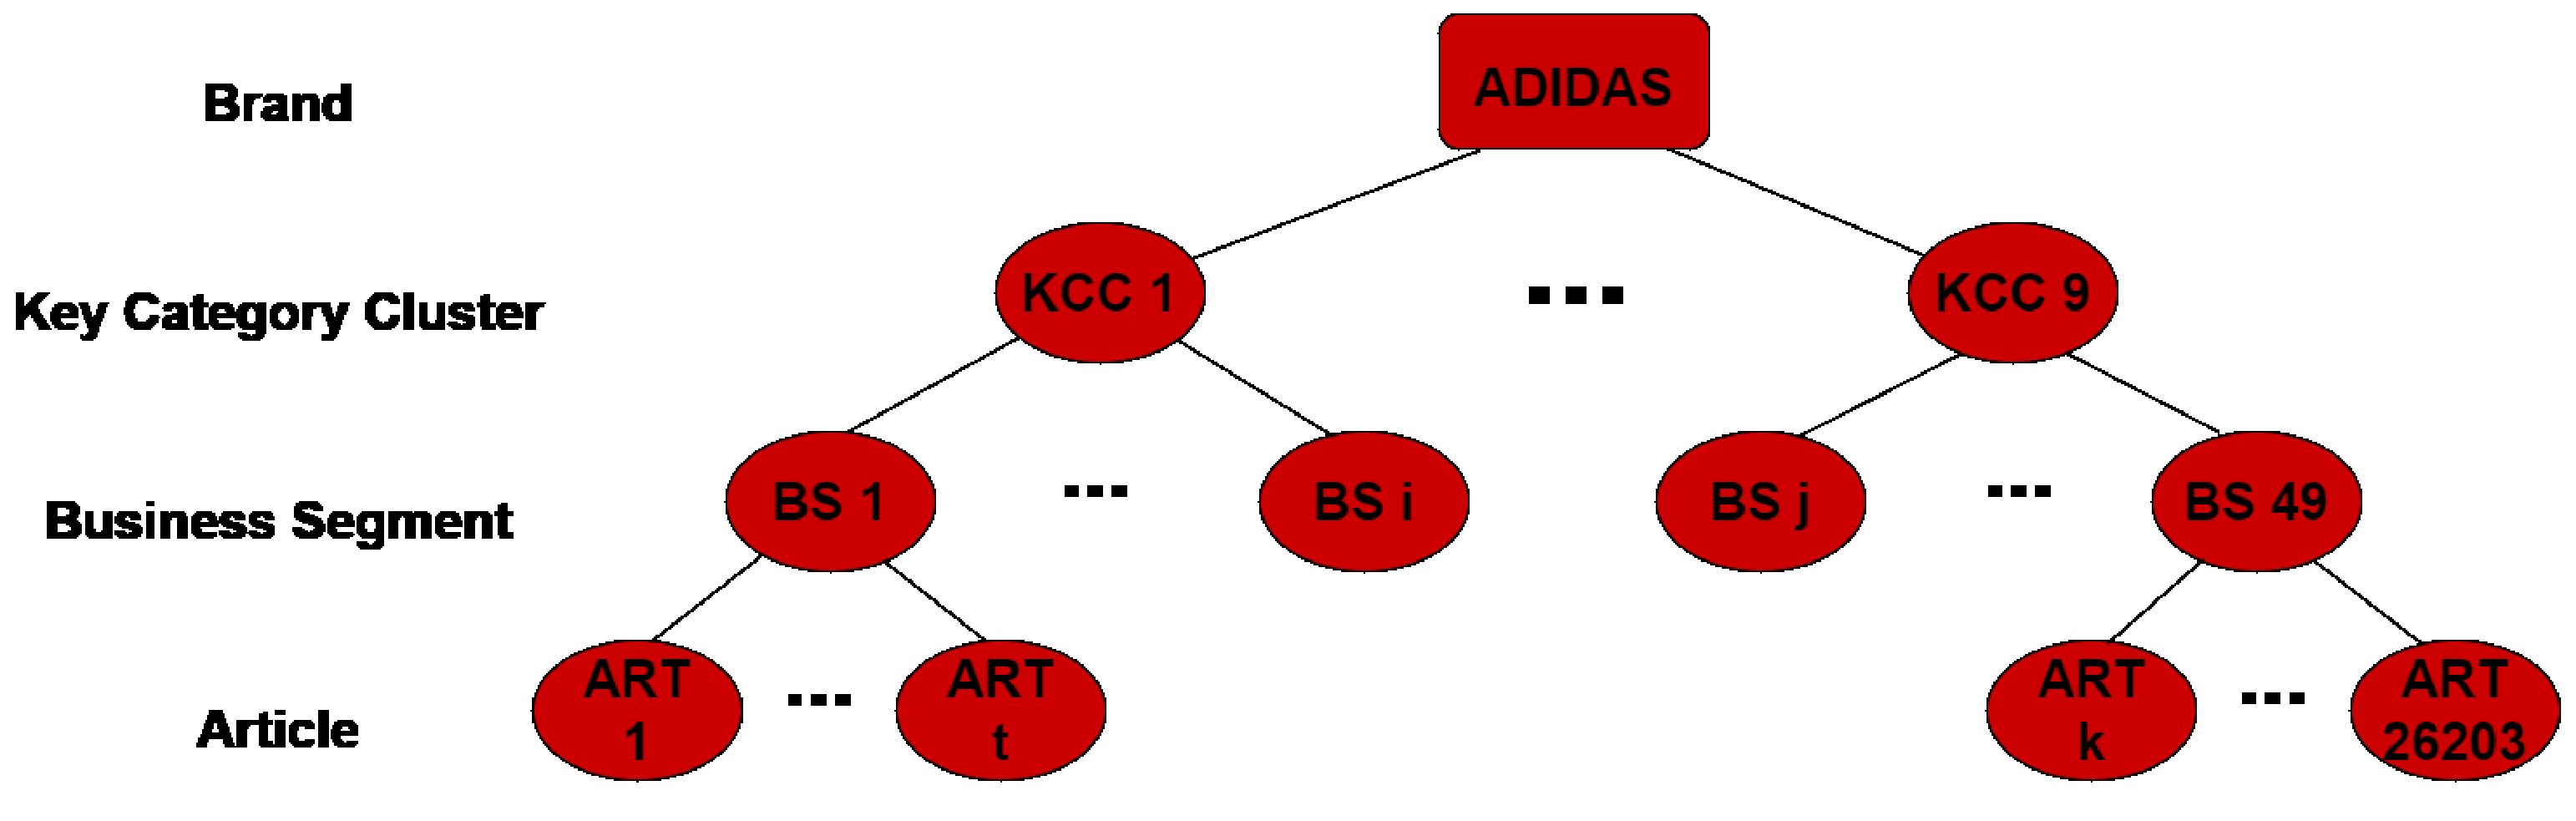
\includegraphics[width=0.95\linewidth]{figures/article_tree_KCC_BS.eps}
  \caption{Illustration of a hierarchical article structure}
  \label{fig:article_hierarchy}
\end{figure}

Worth mentioning is that it is possible that some individual nodes might have only one single child node, meaning that the hierarchy level can stay consistent across multiple nodes. This phenomenon however is very rare and when it occurs, it affects usually two consecutive nodes only. For example, \textit{Sub-Brand 4} has only one child node \textit{KCC 6} (See \autoref{fig:single_childnode}). Sub-Brands are visible for consumers through an own, not shared logo (See \autoref{fig:adidas_logos}).\\

\begin{figure}[H]
\centering
  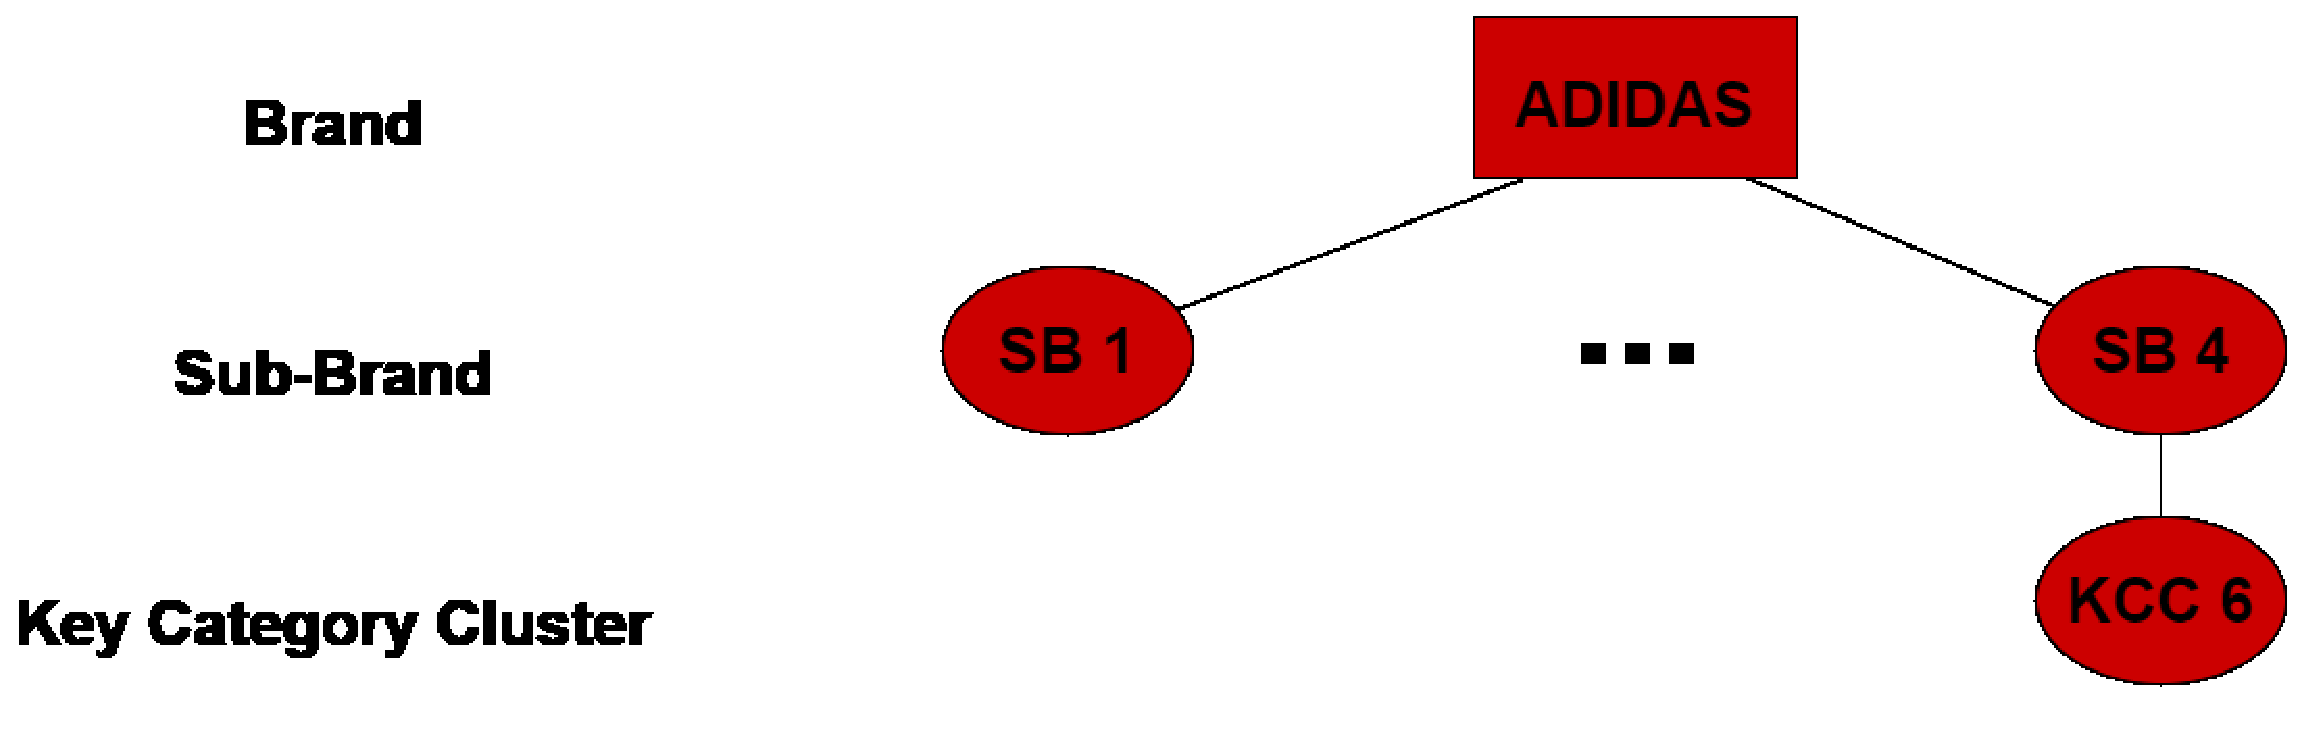
\includegraphics[width=.7\linewidth]{figures/article_tree_single_childnode.eps}
  \caption{Example of a single child node}
  \label{fig:single_childnode}
\end{figure} 










